\section{Laika on Distributed Memory}
\label{sec:partitions}

In this section, we discuss a technique for executing \proc{Laika}
on a distributed memory system.  First, we observe that reordering the vertices
according to the Hilbert priority function, as discussed in \secref{reordering}, 
yields a data layout that
is convenient for distributed memory, following from the same logic that
gives it good cache locality.  That is, the vertex set associated with
each node is essentially a large cache such that as the memory footprint 
for each node grows the fraction of edges crossing between nodes shrinks.
For instance, by the predicted cache miss rate from Tirthapura et al.~\cite{TirthapuraSeAl06}, a node footprint of 16GB would result in approximately
1/100th of the edges crossing between nodes for any number of nodes.  Intuitively,
we can see why this is so in \figref{hilbert_compact}, where we see 
an example of the general property that any subinterval of the Hilbert curve
corresponds to a compact hypervolume in the corresponding $N$D space.  
This is clear from the construction of the Hilbert curve, as described in
\figref{hilbert_construction}, where each block in the Hilbert
curve shares a face with an adjoining block.  Since vertices are locally 
connected, we expect that the number of edge crossings is proportional to the
(hyper) surface area of the volume, whereas the number of vertices is 
proportional to the actual volume, which is one dimension larger.  As such,
as the subinterval of the Hilbert curve grows the ratio of edge
crossings to vertices shrinks.

\begin{figure}[h]
\centering
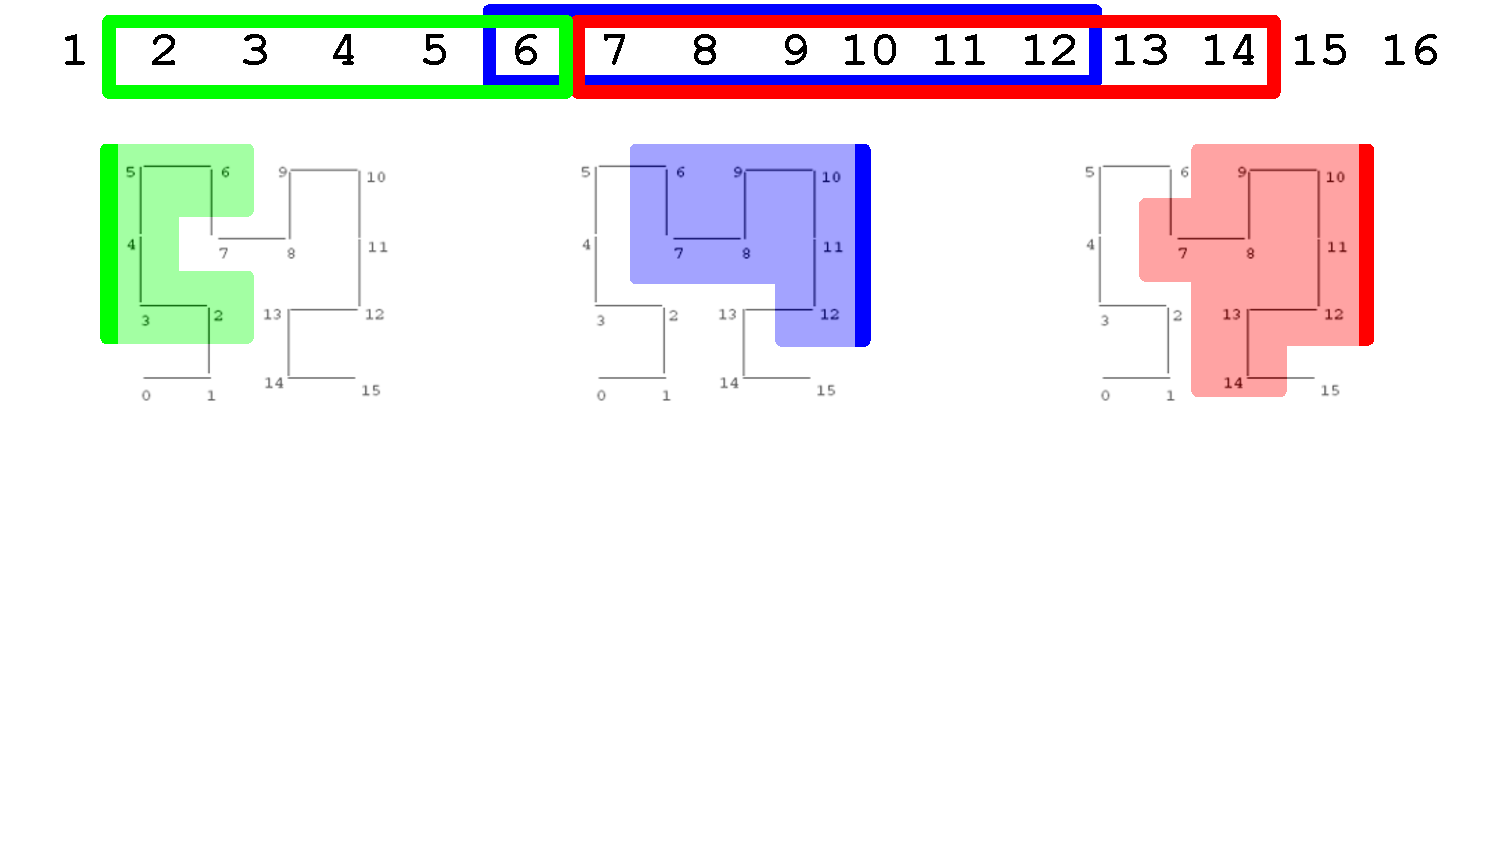
\includegraphics[width=5in,clip,trim=0 6cm 0 0]{figures/hilbert_compact.pdf}
\caption{Examples of how contiguous subintervals yield compact
spaces in 2-dimensional space.}
\label{fig:hilbert_compact}
\end{figure}

\begin{figure}[h]
\centering
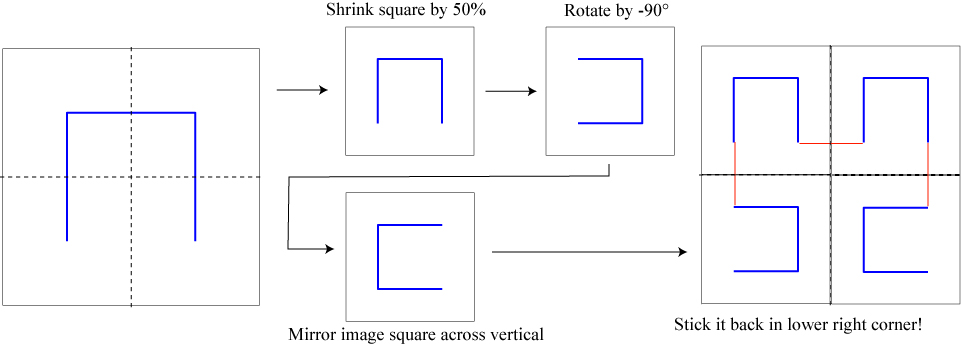
\includegraphics[width=5in,clip,trim=0 0 0 0]{figures/fourthifs.jpg}
\caption{The construction of the Hilbert curve makes it
clear that contiguous subintervals of the curve yields
compact volumes in $N$-dimensional space: the curve always
makes 90 degree turns in an $N$-dimensional construction,
thus every pair of adjacent volumes in the Hilbert curve share a
face.}
\label{fig:hilbert_construction}
\end{figure}

\subsection{Experimental Results}
\label{sec:mpi_empirical}


A simple extension to \proc{Laika} accommodates execution in a distributed
memory system using the message-passing interface (MPI)~\cite{MPI94}.  
We merely divide up the vertices into $R$ (for \emph{ranks}
in the MPI vernacular) contiguous regions and assign each to a rank.  As a 
preprocessing step, one can find all of the edges in the edge set $E$ 
that cross between ranks
and execute the associated communication using MPI, instead of reads and
writes in shared memory.  We allocate a dedicated network thread who sends
updated vertex state for a local vertex $v$ to all ranks who own a vertex
$w$ such that $(v,w) \in E$.  In addition, the network thread also receives
updated vertex state for $w$ and updates associated counters for all
$v$ such that $(v,w) \in E$ and $w$ is a predecessor of 
$v$ (i.e. $\rho(w) < \rho(v)$).  Communication between the network thread
and the workers is accomplished through a pair of concurrent 
queues~\cite{MichaelSc96}.

\begin{wrapfigure}{r}{.5\textwidth}
\centering
\begin{tabular}{c|c}
MPI Ranks & Time (s) \\
\hline
  1 & 64.18 \\
  2 & 38.37 \\
  3 & 27.70 \\
  4 & 23.07 \\
  5 & 20.33 \\
  6 & 17.99 \\
  7 & 16.88 \\
  8 & 15.54 \\
\end{tabular}
\caption{Results of distributed memory experiment executing
\proc{Laika} extended using MPI on up to 8 individual
12-core Intel Xeons.}
\label{fig:mpi_results}
\end{wrapfigure}



We tested this distributed memory version of \proc{Laika} using a set
of 8 Intel Xeons, each with 12 processor cores connected by gigabit ethernet.
In particular, we performed a strong-scaling test of the 50M vertex graph
described in \secref{empirical}.  The strong-scaling results serve as
a worst case for the typical scenario for Simit-generated graphs, which 
would use distributed memory primarily to execute on ever-larger graphs
(i.e. weak-scaling).  However, to give fair scaling results
we adjusted the amount of
work in the \proc{Update} function to reflect the typical amount of work
in a Simit program, which generally performs a 3x3 matrix multiplication
per neighbor in the graph.  In \figref{mpi_results} we see the results of
our experiment, where each rank is executed in paralles on 11 cores (i.e.
the 12th core is used for the network thread) and we scale up to 8
multi-core ranks.  We get approximately a 4x speedup on 8 ranks and a 2.78x
speedup on 4 ranks.  Relatively little performance engineering has been
applied to this implementation, so we suspect that further gains are 
possible.  In addition, we are applying this algorithm to a comparatively
small graph of roughly 1GB.  In practice, Simit will generate graphs that are
approximately the size of main memory, which will also help our scalability.




% In this section, we will describe how the Hilbert curve is also
% a convenient mechanism for paritioning locally connected graphs
% that are embeddable in a low-dimensional space.  That is, it 
% generates a partition with small edge cuts.  We will discuss how
% the priority-dag scheduling approach enables us to decompose the 
% problem into two phases.  The first phase is to extend \proc{Prism}
% to support a reshuffling operator, given a priority value from each
% vertex, which re-organizes the graph data structure in linear order 
% according to the priority function.  The second phase is to partition
% the $n$ vertices by merely assigning $n/p$-sized compact subintervals
% of vertices to each of the $p$ multi-core nodes.  Finally, we 
% will describe the software architecture that integrates MPI commands
% communicating over edges spanning partitions with the priority-dag 
% scheduled computations on each multi-core node.  We will test the
% performance of our implementation by measuring strong-scaling
% performance on a small set of test graphs.


% \section{Dealing with Distributed Execution}
% Since an update function can only be run on a vertex if its 
% neighbors are at most one iteration behind, we need to incur 
% network traffic on every iteration to communicate vertex values 
% for edges that cross machines. This can be done in a few ways. 
% First, when an update function is being run on a vertex, it can 
% fetch the values for neighbors on different machines and then 
% run the necessary computation. This synchronous approach seems 
% less than ideal, since the network traffic falls on the critical 
% path of the iteration -- it is very likely that vertices that 
% are capable of being updated without any network requests are 
% waiting idle as the network requests complete.

% Thus, an asynchronous approach is generally preferable. Our 
% approach is as follows. For each edge that crosses machines, 
% we declare one endpoint vertex as the predecessor and the other 
% as the successor. Once the predecessor is updated, it sends 
% its value to the machine to which the successor is assigned. 
% Once the successor has received values from all of its 
% predecessors, it can be scheduled for execution. If our 
% partioning of vertices across machines is good and there are 
% many vertices on each machine that have no dependencies on 
% external vertices and therefore can be scheduled at any time, 
% then there will be minimal waiting for network messages. Our 
% scheme ensures that we satisfy the constraint that vertex 
% updates must appear to be processed in some global order -- 
% in other words, both of the endpoints of an edge cannot be 
% updated in some iteration based on the other's data from 
% the previous iteration.

% % \begin{figure}[!t]
% % \centering
% % 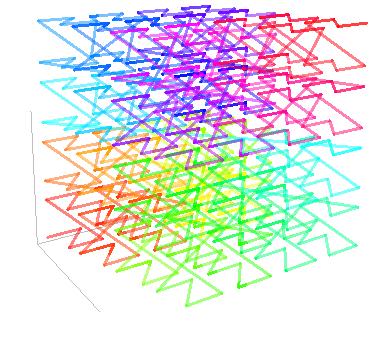
\includegraphics[width=2.5in]{z}
% % \caption{A Z-order curve tracing out the 3D space bounded by the box.}
% % \label{fig_z}
% % \end{figure}

% We partition vertices across machines using a technique 
% based on space-filling curves. A 3D space-filling curve 
% maps the real numbers to points in 3D space so that for 
% an arbitrary point $p$ as we trace out more and more of 
% the curve the distance from $p$ to the nearest point on 
% the curve becomes smaller and smaller. We use a Z-order 
% curve, which has the property that if two points on the 
% curve are relatively close together, then the real numbers 
% that generated those points tend to be relatively close. A 
% Z-order curve in 3D space is shown in Figure 2.

% Each vertex in a mesh graph can be assigned a particular 
% coordinate in 3D space. Thus, we can draw a bounding box 
% in 3D space around a mesh graph. We trace out a Z-order 
% curve over a finite portion of its domain mapping to points 
% n the bounding box. We then assign each vertex in the mesh 
% to its nearest point in the traced curve and mark the vertex 
% with the real number that generated this point, which we will 
% call the Z-number. We then sort the vertices by Z-number. 
% Nearby vertices in the sorted order should be nearby in the 
% physical graph. We can then split this sorted list into 
% contiguous chunks, one for each machine in our cluster. 
% Since each chunk should correspond to some contiguous 
% region in 3D space, the number of edges crossing machines 
% should be fairly small, as explained in the previous section.
